\section{Variables}
\label{sec:var}
\begin{frame}<beamer>
    \frametitle{Outline}
    \tableofcontents[currentsection]
\end{frame}

\begin{frame}[fragile]
\frametitle{Variable Types and Operations}
\begin{itemize}
	\item {Try following code:}
\begin{lstlisting}[xleftmargin=0.05\linewidth, linewidth=0.9\linewidth]
#include <stdio.h>
int main( )
{
  int a = 5, b = 3;
  float val1 = a/b;
  float val2 = (float)(a/b);
  float val3 = (float)(a+0.0)/b;
  printf("a/b is: val1 = %f\n", val1);
  printf("a/b is: val2 = %f\n", val2);
  printf("a/b is: val3 = %f\n", val3);
}
\end{lstlisting}
\end{itemize}
\end{frame}

\begin{frame}[fragile]
\frametitle{Character and String}
\vspace{-0.14in}
\begin{itemize}
	\item {Try following code:}
\begin{lstlisting}[xleftmargin=0.05\linewidth, linewidth=0.9\linewidth]
#include <stdio.h>
int main()
{
   char *str1 = "abc\0de";
   char *str2 = "abc\rde";
   char *str3 = "abc\tde";
   char *str4 = "abc\t\b\b\b\b\bde";
   char ch1 = 'A'+6;
   char ch2 = 'A' + 'B';
   printf("%s\n", str1);
   printf("%s\n", str2);
   printf("%s\n", str3);
   printf("%s\n", str4);
   printf("%c, value=%d\n", ch1, ch1);
   printf("%c, value=%d\n", ch2, ch2);
}
\end{lstlisting}
\end{itemize}
\end{frame}

\begin{frame}[fragile]{How Variable Behaves}
\begin{itemize}
	\item {Guess the values of \textbf{a}, \textbf{i} and \textbf{j}}
	\item {Try following code to verify your answer:}
\end{itemize}

\begin{lstlisting}
#include <stdio.h>
int main()
{
   int  i = 4, j = 6;
   int  a = i + j;
   printf("a = %d\n", a);
   i = j - i; 
   j = i + j;
   printf("i = %d, j = %d\n", i, j);
}
\end{lstlisting}
\end{frame}

\begin{frame}[fragile]
\frametitle{printf() and Precision Control}
\begin{itemize}
	\item {Given float number \textcolor{red}{a = 231.36952}, integer number \textcolor{red}{b = 39} and integer number \textcolor{red}{c=0xEE}}
	\begin{enumerate}
		\item{Print out \textcolor{red}{a} with \textcolor{red}{2} digits precision and \textcolor{red}{3} digits precision respectively}
		\item{Print out octal and hexadecimal values of \textcolor{red}{b}}
		\item{Print out decimal and octal nunmber of \textcolor{red}{c}}
	\end{enumerate}
\end{itemize}

\begin{lstlisting}[xleftmargin=0.08\linewidth, linewidth=0.9\linewidth]
#include <stdio.h>
int main( )
{
   float a = 231.36952;
   int b = 39;
   int c = 0xEE;
}
\end{lstlisting}
\end{frame}

\ifx\answer\undefined
\begin{frame}[fragile]
\frametitle{printf() and Precision Control: the answer}
\begin{itemize}
	\item {Try following code:}
	\begin{lstlisting}[xleftmargin=0.08\linewidth, linewidth=0.9\linewidth]
#include <stdio.h>
int main( )
{
   float a = 231.36952;
   int b = 39;
   int c = 0xEE;
   printf("a = %3.2f\n", a);
   printf("a = %3.3f\n", a);
   printf("b = %0x\n", b);
   printf("b = %o\n",  b);
   printf("c = %d\n", c);
   printf("c = %o\n", c);
}
	\end{lstlisting}
\end{itemize}
\end{frame}
\fi

\begin{frame}[fragile]
\frametitle{Print out the values of different variables}
\vspace{-0.1in}
\begin{itemize}
	\item {Given following variables have been defined}
	\item {Please show the number of bytes they occupy in the memory}
\end{itemize}
\begin{lstlisting}[xleftmargin=0.08\linewidth, linewidth=0.96\linewidth]
#include <stdio.h>
int main()
{
   char ch = 'B';
   int  a  = 0;
   short b = 1024;
   double c = 0.1;
   float d = 22;
   double e = 3.1415926;
}
\end{lstlisting}
\vspace{-0.2in}
\begin{itemize}
	\item {Please print the values of different variables on the screen}
	\item {For example,}
\end{itemize}
\begin{lstlisting}[xleftmargin=0.08\linewidth, linewidth=0.96\linewidth]
   printf("%f\n", d);
\end{lstlisting}
\end{frame}

%\ifx\answer\undefined
\begin{frame}[fragile]
\frametitle{Precision of \textcolor{blue}{float} and \textcolor{blue}{double}}
\vspace{-0.1in}
\begin{lstlisting}[xleftmargin=0.08\linewidth, linewidth=0.96\linewidth]
#include <stdio.h>
int main()
{
   double c = 0.1;
   float d = 22;
   double e = 3.1415926;
   printf("e = %1.4lf\n", e);
   printf("e = %1.3lf\n", e);
   printf("e = %1.2lf\n", e);
}
\end{lstlisting}
\end{frame}
%\fi

\begin{frame}[fragile]{Print integer numbers with formating}
\begin{itemize}
	\item {Print out a=234, b=5, c=123, d=55, two numbers in each line}
	\item {Numbers are separated by `, '}
	\item {Each number occupy 6 digital position, right-aligned}
\end{itemize}
\begin{figure}
	\centering
	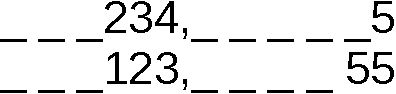
\includegraphics[width=0.5\linewidth]{figs/format.pdf}
\end{figure}
\end{frame}

%\ifx\answer\undefined
\begin{frame}[fragile]{Print integer numbers with right-aligned}
\begin{itemize}
	\item {Try following code:}
\end{itemize}

\begin{lstlisting}
#include <stdio.h>
int main()
{
   int a = 234;
   int b = 5;
   int c = 1231;
   int d = 55;
   printf("%6d, %6d\n", a, b);
   printf("%6d, %6d\n", c, d);
}
\end{lstlisting}
\end{frame}
%\fi

\begin{frame}[fragile]{Print integer numbers with left-aligned}
\begin{itemize}
	\item {Try following code:}
\end{itemize}

\begin{lstlisting}
#include <stdio.h>
int main()
{
   int a = 234;
   int b = 5;
   int c = 1231;
   int d = 55;
   printf("%-6d, %-6d\n", a, b);
   printf("%-6d, %-6d\n", c, d);
}
\end{lstlisting}
\end{frame}